\documentclass[abstracton,12pt]{scrartcl}
    
\usepackage[utf8]{inputenc}
% \usepackage[T1]{fontenc}
\usepackage{fancyhdr}
\usepackage{graphicx}
\usepackage{tikz}
\usepackage{listings}
\usepackage{amssymb}
\usepackage{amsfonts}
\usepackage{amsmath}
\usepackage{amsthm}
\usepackage{pdfpages}
\usepackage{forest}
\usepackage{multicol}
\usepackage{varwidth}
\usepackage{verbatim}
\usepackage{cleveref}
\usepackage{minted}
\usepackage[ruled,vlined]{algorithm2e}
\usepackage{caption}
\usepackage{subcaption}
\usepackage{soul}
\usepackage{microtype}
\usepackage{pgfplots}
% \usepackage{ulem}
% \usepackage{ifthen}
% \usepackage{wrapfig}
% \usepackage{geometry}
% \usepackage{titlesec}

\forestset{qtree/.style={for tree={parent anchor=south, child anchor=north,align=left,inner sep=0pt}}}
\graphicspath{ {images/} }
\pgfplotsset{yticklabel style={text width=2.5em,align=right}}
% \setlength{\multicolsep}{6.0pt plus 2.0pt minus 1.5pt}% 50% of original values
% \titleformat{\chapter}{}{\thechapter}{}{}
% \titlespacing{\chapter}{-100pt}{-100pt}{-100pt}

% --------- 

\titlehead{Department of Informatics, University of Zürich}
\subject{\vspace*{2cm}MSc Basismodul}
\title{The Adaptive Radix Tree}
\author{
    Rafael Kallis\\[-5pt]
    \scriptsize Matrikelnummer: 14-708-887\\[-5pt]
    \scriptsize Email: \texttt{rk@rafaelkallis.com}
}
\date{\vspace*{2cm}September 1, 2018}
\publishers{
    \small supervised by Prof.\ Dr.\ Michael\ Böhlen and Kevin\ Wellenzohn \\[5cm]
    \begin{tikzpicture}[overlay]
    \node at (-3,-3) {
\includegraphics[height=1.5cm]{IFIlogo}};
    \node at (7,-3) {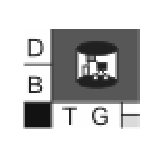
\includegraphics[height=1.5cm]{dbtgBW}};
    \end{tikzpicture}
}

% \dedication{dedicated to xxx}

% --------- 

\theoremstyle{definition}

\newtheorem{definition}{Definition}
% \newtheorem{figure}{Figure}
\newtheorem{example}{Example}
% \newtheorem{theorem}{Theorem}
% \newtheorem{lemma}{Lemma}

\crefname{algocfline}{algorithm}{algorithms}
\Crefname{algocfline}{Algorithm}{Algorithms}

\crefname{figure}{Fig.}{Figs.}
\Crefname{figure}{Figure}{Figures}

\crefname{example}{Ex.}{Ex.}
\Crefname{example}{Example}{Examples}

% \newenvironment{proof}
%     {\noindent{\bf Proof:\rm}}{\hfill$\Box$\vspace{\medskipamount}}

\newenvironment{centerverbatim}{\par\centering\varwidth{\linewidth}\verbatim}
    {\endverbatim\endvarwidth\par}

\def\bbbr{{\rm I\!R}}
\def\bbbm{{\rm I\!M}}
\def\bbbn{{\rm I\!N}}
\def\bbbz{{\rm I\!Z}}

% --------- 

\begin{document}

\maketitle

% \chapter*{Acknowledgements}

% \begin{abstract}
%   ...
% \end{abstract}

% \chapter*{Zusammenfassung}

% \tableofcontents
% \listoffigures
% \listoftables

\newpage
\section{Introduction}

Main-Memory Databases increasingly become a viable option for many applications
due to the considerably faster access times of volatile memory 
in comparison to secondary storage.

Leis et al.\ \cite{leis2013adaptive} propose the Adaptive Radix Tree (ART), an in-memory
data structure which efficiently stores and retrieves data.
As we will see later, ART achieves its performance, and space
efficiency, by compressing the tree both vertically and horizontally.

The goal of this project is to study and implement ART, as proposed by 
\cite{leis2013adaptive}. 
In \Cref{sec:art} we describe how ART is constructed by applying 
vertical and horizontal compression to a trie.
Next, we describe the point query procedure, as well as 
key deletion in \Cref{sec:algorithms}.
Finally, a benchmark of ART, a red-black tree and a hashtable
is presented in \Cref{sec:benchmarks}.

\section{Preliminaries}
\label{sec:preliminaries}

A trie \cite{fredkin1960trie} is a hierarchical data structure which
stores key-value pairs. Tries can answer both point and range queries 
efficiently since keys are stored in lexicographic order.
A node's key can be reconstructed from its path and therefore, when 
constructing a trie from a set of keys, all insertion orders result in the 
same tree. Tries do not require rebalancing operations and therefore have 
no notion of balance, unlike comparison based search trees.

Keys are split into chunks of $s$ bits, where $s$ is called \textit{span}.
Inner nodes have  $2^s$ child pointers (possibly \texttt{null}), 
one for each possible $s$-bit sequence. During tree
traversal, we propagate down to the child node identified by the $d$-th
$s$-bit chunk of the key, where $d$ is the depth of the current node. 
Using an array of $2^s$  pointers, this lookup can be done without any 
additional comparison. 

\Cref{fig:span} depicts tries storing the 
8-bit keys ``$01000011$'', ``$01000110$'' and ``$01100100$'' with 
$s=1,2$. Span $s$ is critical for the performance of the trie because $s$ 
determines the height of the trie. We observe that by increasing the span, 
we decrease the tree height. A trie
storing $k$ bit keys has $\lceil \frac{k}{s} \rceil$ levels of inner nodes.
As a consequence, point queries, insertions and deletions have 
$O(k)$ complexity.

Span $s$ also determines the space consumption of the tree.
A node with span $s$ requires $2^s$ pointers. 
An apparent trade off exists between tree height versus space efficiency that
depends on $s$.

\begin{figure}[h]
  \centering
  \begin{subfigure}[b]{0.4\textwidth}
    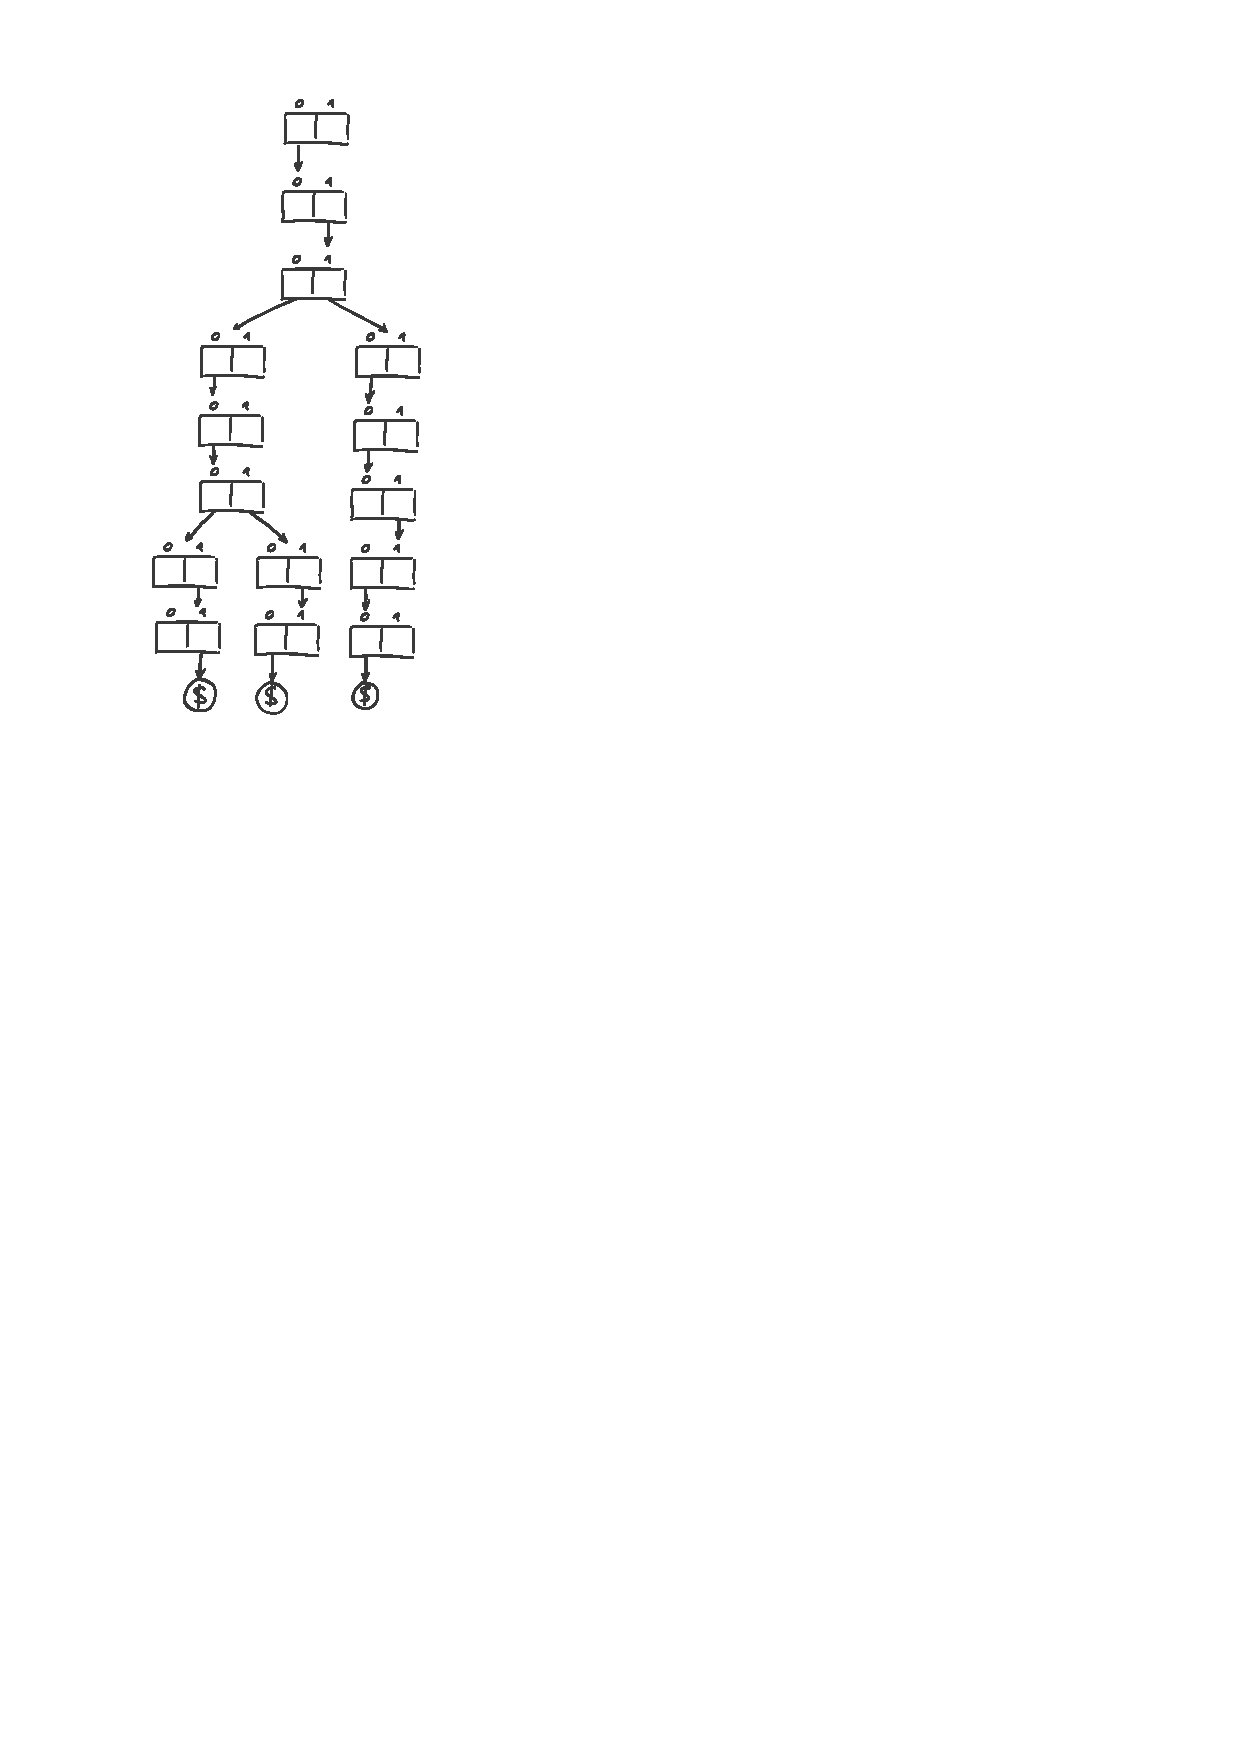
\includegraphics[height=10cm,trim={2cm 17.5cm 2.5cm 1.5cm},clip]{trie_s1_draw}
    \caption{$s=1$}
  \end{subfigure}
  \begin{subfigure}[b]{0.55\textwidth}
    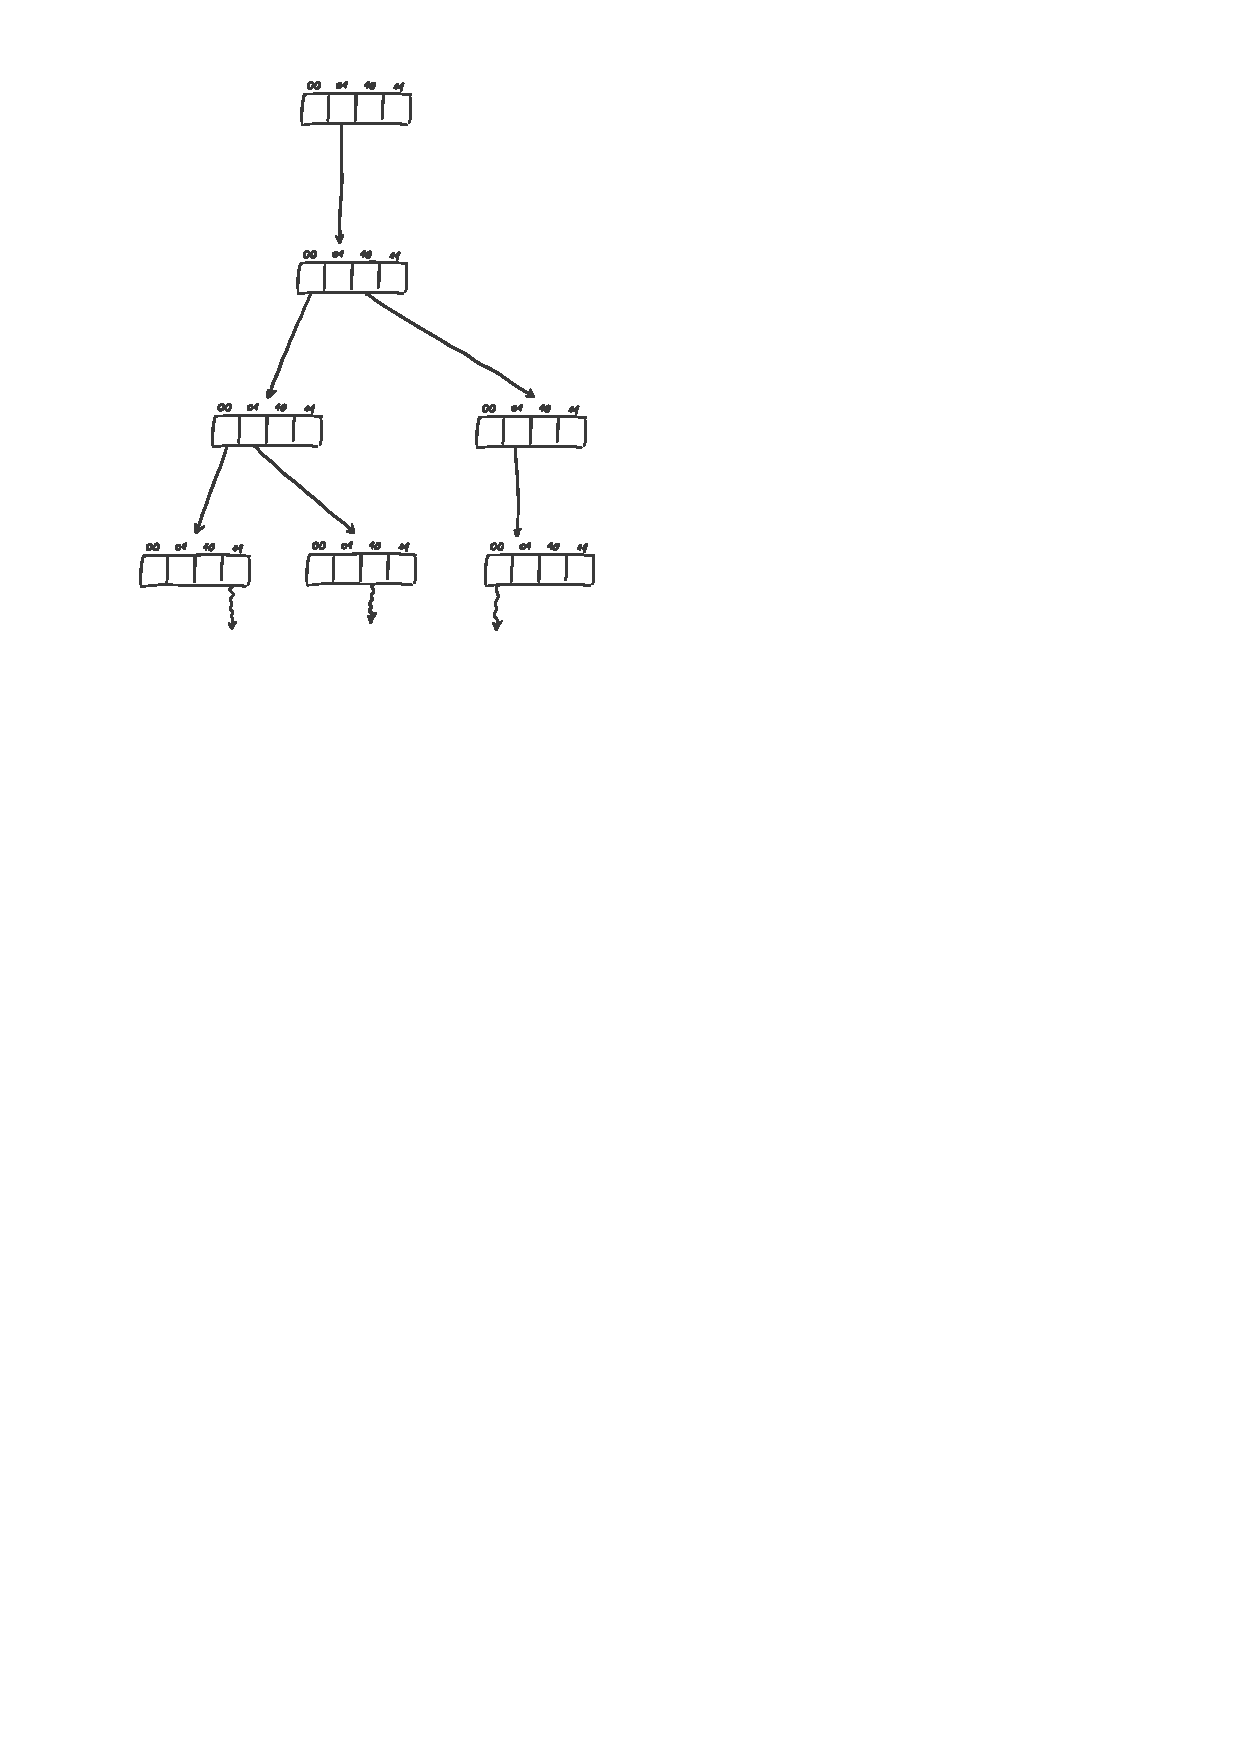
\includegraphics[height=10cm,trim={2cm 18.5cm 2.5cm 0.5cm},clip]{trie_s2_draw}
    \caption{$s=2$}
  \end{subfigure}
  \caption{
    Tries with span $s=1,2$ storing keys ``$01000011$'', ``$01000110$''
    and ``$01100100$''.
  }
  \label{fig:span}
\end{figure}

\newpage

\section{Adaptive Radix Tree (ART)}
\label{sec:art}

The \textit{Adaptive Radix Tree} (ART) is a space efficient trie, which
achieves its low memory consumption using \textit{vertical} and 
\textit{horizontal} compression. Using vertical compression, ART reduces
the tree height significantly by merging parent nodes with child nodes
under certain circumstances. Horizontal compression reduces the amount
of space required by each node depending on the number of child nodes.

\subsection{Vertical (Prefix) Compression}
\label{sec:vertical-compression}

When storing long keys, chains of nodes start to form where each node only
has a single child. As a consequence, a lot of space is wasted as many nodes
with little actual content are kept and traversals are slowed down because
many nodes are traversed. Space wasting is further amplified with sparse
datasets or a small span.

Morrison introduced \textit{Patricia}~\cite{morrison1968patricia}. 
Patricia is a space-optimized trie in which
each node with no siblings is merged with its parent, i.e.\ inner nodes
are only created if they are required to distinguish at least two leaf nodes. 
Doing so, chains caused by long keys are eliminated, which make tries 
space-inefficient. Although Morrison's Patricia tree is a bitwise trie, i.e.\ 
has a span $s=1$, the technique can be applied to tries with any span.
We refer to this technique as \textit{vertical compression}.

Vertical compression is implemented by storing an additional variable, called
\textit{prefix}, inside each node. This variable stores the concatenation
of partial keys of descendants that were eliminated because they had no 
siblings. \Cref{fig:vertical-compression} depicts two tries, one with and one 
without vertical compression. We observe that nodes with no siblings, color 
coded red, are eliminated and their partial key is appended to the parent's 
prefix. 

\begin{figure}[h]
  \begin{footnotesize}
    \begin{multicols}{2}
      \noindent
      \begin{flushright}
      \framebox(160,160){
        \begin{forest}
          [,circle,draw
            [,circle,draw,red, edge label={node[midway,right,font=\footnotesize]{$01$}}
              [,circle,draw, edge label={node[midway,left,font=\footnotesize]{$00$}}
                [,circle,draw, edge label={node[midway,left,font=\footnotesize]{$00$}}
                  [,circle,draw,red, edge label={node[midway,left,font=\footnotesize]{$11$}}]
                ]
                [,phantom]
                [,circle,draw, edge label={node[midway,right,font=\footnotesize]{$01$}}
                  [,circle,draw,red, edge label={node[midway,right,font=\footnotesize]{$10$}}]
                ]
              ]
              [,phantom]
              [,phantom]
              [,circle,draw, edge label={node[midway,right,font=\footnotesize]{$10$}}
                [,circle,draw,red, edge label={node[midway,right,font=\footnotesize]{$01$}}
                  [,circle,draw,red, edge label={node[midway,right,font=\footnotesize]{$10$}}]
                ]
              ]
            ]
          ]
        \end{forest}
      }
      \hspace{5mm}
      \end{flushright}
      ~

      \begin{flushleft}
      \hspace{5mm}
      \framebox(160,160){
        \begin{forest}
          [,circle,draw
            [,circle,draw, edge label={node[midway,left,font=\footnotesize]{$00$}}
              [,circle,draw, edge label={node[midway,left,font=\footnotesize]{$00$}}]{
                \draw[gray] (.east)--++(0.5em,0em)
                  node[anchor=west,gray]{11};
              }
              [,phantom]
              [,circle,draw, edge label={node[midway,right,font=\footnotesize]{$10$}}]{
                \draw[gray] (.east)--++(0.5em,0em)
                  node[anchor=west,gray]{01};
              }
            ]
            [,phantom]
            [,phantom]
            [,circle,draw, edge label={node[midway,right,font=\footnotesize]{$10$}}]{
              \draw[gray] (.east)--++(0.5em,0em)
                node[anchor=west,gray]{0110};
            }
          ]{
            \draw[gray] (.east)--++(0.5em,0em)
              node[anchor=west,gray]{01};
          }
        \end{forest}
      }
      \end{flushleft}
    \end{multicols}
  \end{footnotesize}
  \caption{
    Tries with span $s=2$ storing keys ``$01000011$'', ``$01000110$''
    and ``$01100100$''. The trie on the right incorporates vertical 
    compression. Red nodes indicate nodes which get eliminated under
    vertical compression. Gray strings represent the value of the prefix 
    variable.
  }
  \label{fig:vertical-compression}
\end{figure}

\subsection{Horizontal Compression (Adaptive Nodes)}
\label{sec:horizontal-compression}

With large values of span $s$, an excessive amount of space is sacrificed
to achieve a smaller tree height. Space is allocated for pointers which keep
references to child nodes, even if they are unused.

In order to reduce the space needed to keep
such references, Leis et al.\ propose \textit{Adaptive Nodes} 
\cite{leis2013adaptive}, which make use of dynamic data structures 
instead of static arrays for child node bookkeeping. Doing so, we allocate 
a minimal amount of space when the number of children is small and add more 
space if required, i.e.\ more children are added.
We refer to this technique as \textit{horizontal compression}.
Leis et al.\ fix the span $s=8$, i.e. partial keys are 1 byte
long and therefore each node can have up to $2^8 = 256$ children.

When applying horizontal compression, a node is in one of four configurations, 
depending on the number of child nodes. Each of the four configurations is 
optimized for a different amount of children.
When keys are inserted/deleted, the nodes are adapted accordingly.
The most compact configuration 
is called \texttt{Node4} which can carry up to four children. 
In the same manner, we also have \texttt{Node16}, \texttt{Node48} 
and \texttt{Node256}. All nodes have a header which stores the node type,
the number of children and the prefix variable, which contains the compressed
path (c.f.\ \Cref{sec:vertical-compression}).

\begin{figure}[h]
  \centering
  \begin{tabular}{ l|r|r } 
    Type & Children & Space (bytes) \\
    \hline
    \texttt{Node4} & 2-4 & $h + 4 + 4 \cdot 8 = h + 36$ \\ 
    \texttt{Node16} & 5-16 & $h + 16 + 16 \cdot 8 = h + 144$ \\ 
    \texttt{Node48} & 17-48 & $h + 256 + 48 \cdot 8 = h + 640$ \\ 
    \texttt{Node256} & 49-256 & $h + 256 \cdot 8 = h + 2048$ 
  \end{tabular}
  \caption{Space consumption for each inner node type. $h$ is equal to
    the size of the header.}
  \label{fig:node-sizes}
\end{figure}

We now describe the structure of each of the four configurations.
\Cref{fig:node-sizes} shows the space consumption for each inner node type.
Note that $h$ is equal to the header's size.
\Cref{fig:horizontal-compression} illustrates the state of a node
for each node type,
when storing the partial keys $65$, $82$, $84$ and pointers to their 
corresponding child nodes $\alpha$, $\beta$, $\gamma$. 
Note that $\varnothing$ represents a \texttt{null} pointer.

A node of type \texttt{Node4} contains two 4-element arrays, one called
``partial keys'' and one called ``children''.
The ``partial keys'' array, holds
partial keys which identify children of that node. 
The ``children'' array, holds pointers to the child nodes.
Partial keys and pointers are stored at corresponding positions and
the partial keys are sorted.

A node of type \texttt{Node16} is structured similarly
to \texttt{Node4}, the only difference being the lengths of the two static 
arrays, which are 16 each.

An instance of \texttt{Node48} contains a 256-element array named 
``indexes'' and a 48-element array called ``children''.
Partial keys are stored implicitly in ``indexes'', i.e.\ 
can be indexed with partial key bytes directly.
As the name suggests, ``indexes'' stores the index of a child
node inside the ``children'' array. This node can be compared to
virtual memory, since the address space (256 addresses) is wider 
than the actual available storage space (48 slots).

Finally, a node of type \texttt{Node256} contains an array of
256 pointers which can be indexed with partial key bytes directly.
Child nodes can be found with a single lookup.

\begin{figure}[h!]
  \centering
  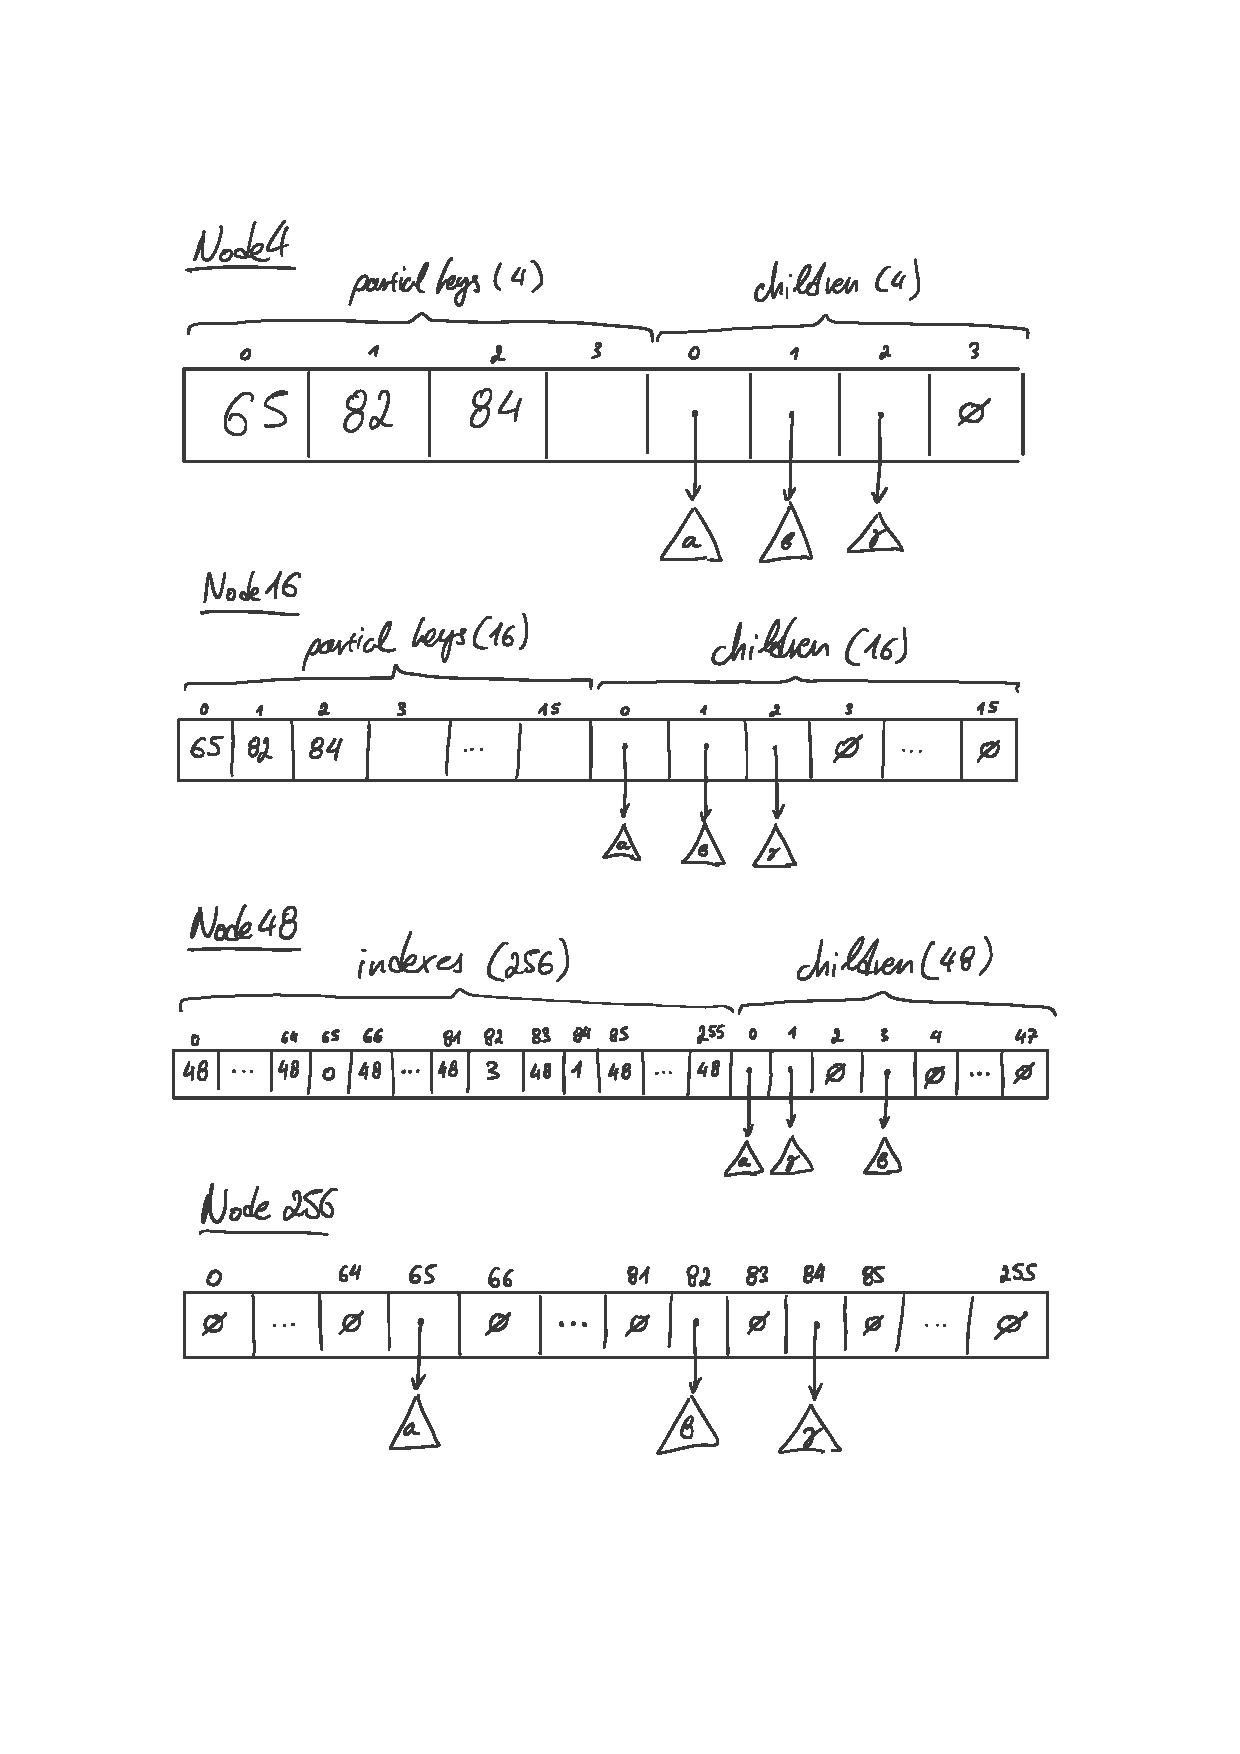
\includegraphics[height=20cm,trim={2.5cm 5cm 2.5cm 3.5cm},clip]{art_nodes_draw}
  \caption{
    When horizontal compression is applied, a node is in one of four 
    configurations, namely \texttt{Node4}, \texttt{Node16}, \texttt{Node48} 
    and \texttt{Node256}.
    Each of the four configurations is optimized for a different number of 
    child nodes. We store the partial keys $65$, $82$, $84$ and their 
    corresponding child nodes $\alpha$, $\beta$, $\gamma$ in an instance
    of each node type. Note that $\varnothing$ represents a \texttt{null} 
    pointer.
  }
 \label{fig:horizontal-compression}
\end{figure}

\section{Algorithms}\label{sec:algorithms}

We will now describe how two fundamental operations, namely
point query and deletion are implemented in ART.
The algorithms mentioned below are based on the implementations presented by
Leis et al.\ \cite{leis2013adaptive}. Note that our implementation uses
\textit{single-value leaves} (c.f.\ Leis et al.\ \cite{leis2013adaptive}), 
i.e.\ values are stored using an additional leaf node type, conveniently
called \texttt{Node0}, which stores one value. Additionally, we utilize
\textit{pessimistic} vertical compression, i.e.\ each inner node stores
the entire compressed path inside the \texttt{prefix} variable using a variable length
partial key vector. During traversal, \texttt{prefix} is compared to the search key.
We present our implementations below.

\subsection{Point Query}\label{sec:point-query}

The code fragment in \Cref{algo:point-query} shows the implementation of a point query on ART in
C++. Method \texttt{get} accepts a key as an argument and returns a pointer
to the value associated with the given key, or \texttt{null} if the key is not found.

In lines 7-8 we declare and initialize a pointer, \texttt{cur}, which references the
current node during tree traversal, and an integer, \texttt{depth} which holds the depth
of the current node.

We now enter a loop in which we check if \texttt{cur} references \texttt{null}
during the beginning of each iteration, and if so, we return \texttt{null}.

In lines 11-16 we check if a prefix mismatch occurs. This step is required
because of vertical compression (c.f.\ \Cref{sec:vertical-compression}).
Method \texttt{check\_prefix} is a member of the \texttt{node} class which
determines the number of matching bytes between \texttt{cur}'s prefix
and \texttt{key} w.r.t.\ the current depth. If a prefix mismatch is discovered,
\texttt{null} is returned.

Lines 17-21 check for an exact match of the key at the current node. If so,
we return the value of the current node.

Finally, we traverse to the next child node. \texttt{depth} is increased to
account for the nodes merged due to vertical compression.
We lookup the next child node, which is assigned to \texttt{cur}.

\begin{figure}[H]
  \begin{minted}[numbers=left,frame=single,fontsize=\scriptsize]{c++}
template <class T> class art {
public:
  /**
   * Finds the value associated with the given key.
   */
  T *get(const key_type &key) const {
    node<T> *cur = root_;
    int depth = 0;

    while (cur != nullptr) {
      const int prefix_len = cur->get_prefix().length();
      const bool is_prefix_match = prefix_len == cur->check_prefix(key, depth);

      if (!is_prefix_match) {
        return nullptr;
      }
      const bool is_exact_match = prefix_len == key.length() - depth;

      if (is_exact_match) {
        return cur->get_value();
      }
      depth += prefix_len;
      node<T> **next = cur->find_child(key[depth]);
      cur = next != nullptr ? *next : nullptr;
      ++depth;
    }
    return nullptr;
  }

  /* ... */
private:
  node<T> *root_ = nullptr;
}
  \end{minted}
  \caption{Point query implemented in C++.}
  \label{algo:point-query}
\end{figure}

\subsection{Deletion}
\label{sec:deletion}

\Cref{algo:deletion} presents our implementation of key deletion on ART in C++.
During deletion, the leaf node is removed from an inner node, which is shrunk
if necessary. If the leaf to remove only has one sibling, vertical
compression is applied to the parent, effectively deleting it.

In lines 7-11, we declare and initialize two pointers, \texttt{cur} and
\texttt{par} which reference the current and parent node during tree traversal.
Variable \texttt{cur\_partial\_key} holds the partial key which indexes the
current node in the parent's child lookup table.
Variables \texttt{depth} and \texttt{key\_len} hold the depth of the current
node and length of the key, respectively.

Next, we loop until \texttt{cur} is a \texttt{null} pointer. During each
iteration we define the following variables:
\begin{itemize}
  \item \texttt{prefix} compressed path of the current node.
  \item \texttt{prefix\_len} length of the compressed path, i.e.\ the number
    of nodes vertically compressed.
  \item \texttt{is\_prefix\_match} evaluates to true iff \texttt{prefix} is a
    prefix of the search key, starting from position \texttt{depth}
    (e.g.\ if \texttt{prefix} = ``aa'' and \texttt{key} = ``aaa'', then
    $\texttt{is\_prefix\_match} \iff \texttt{depth} > 0 \land \texttt{depth} < 2$).
  \item \texttt{is\_exact\_match} evaluates to true iff \texttt{prefix} matches
    the search key, starting from position \texttt{depth}.
    (e.g.\ if \texttt{prefix} = ``aa'' and \texttt{key} = ``aaa'', then
    $\texttt{is\_exact\_match} \iff \texttt{depth} = 1$).
\end{itemize}

If there is a prefix mismatch, i.e.\ \texttt{is\_prefix\_match} evaluates to
false, the search key is not found and a \texttt{null} pointer is returned.
If there is a exact match i.e.\ \texttt{is\_exact\_match} evaluates to true,
we found the node to delete, otherwise we continue traversing down the tree.

After the node to delete has been found, we first extract its associated value
and determine its number of siblings. It must have at least one sibling, 
unless the node to delete is the root node.

If the node to delete has exactly one sibling (lines 27-41), we replace the 
parent node with the sibling, append to the sibling's prefix the parent's
prefix and the sibling's partial key and then delete the \texttt{cur} and
\texttt{par}. We also delete \texttt{par} because of vertical compression.

If the node to delete has more than one sibling (lines 41-43), then no additional action
is required besides deleting \texttt{cur}.

Lines 45-47 check if the parent node is undefull, i.e.\ requires shrinking
(c.f.\ \Cref{sec:horizontal-compression}).

Finally, the value associated with the deleted node is returned (in case the
procedure callee has to free resources).

\begin{figure}[H]
  \begin{minted}[numbers=left,frame=single,fontsize=\scriptsize]{c++}
template <class T> class art {
public:
  /**
   * Deletes the the given key and returns its associated value.
   */
  T *del(const key_type &key) {
    node<T> **cur = &root_;
    partial_key_type cur_partial_key = 0;
    node<T> **par = nullptr;
    int depth = 0;
    const int key_len = key.length();

    while (*cur != nullptr) {
      const key_type prefix = (*cur)->get_prefix();
      const int prefix_len = prefix.length();
      const bool is_prefix_match = prefix_len == (*cur)->check_prefix(key, depth);

      if (!is_prefix_match) {
        return nullptr;
      }
      const bool is_exact_match = prefix_len == key_len - depth;

      if (is_exact_match) {
        T *value = (*cur)->get_value();
        const int n_siblings = par != nullptr ? (*par)->get_n_children() - 1 : 0;

        if (n_siblings == 1) {
          /* find sibling and compress */
          partial_key_type sibling_partial_key = (*par)->next_partial_key(0);
          if (sibling_partial_key == cur_partial_key) {
            sibling_partial_key = (*par)->next_partial_key(cur_partial_key + 1);
          }
          node<T> *sibling = *(*par)->find_child(sibling_partial_key);
          const key_type new_sibling_prefix = (*par)->get_prefix() +
                                              key_type(1, sibling_partial_key) +
                                              sibling->get_prefix();
          sibling->set_prefix(new_sibling_prefix);
          delete (*par);
          *par = sibling;

        } else if (n_siblings > 1) {
          (*par)->del_child(cur_partial_key);
        } 

        if (par != nullptr && (*par)->is_underfull()) {
          *par = (*par)->shrink();
        }
        delete(*cur);
        *cur = nullptr;
        return value;
      }
      cur_partial_key = key[depth + prefix_len];
      par = cur;
      cur = (*cur)->find_child(cur_partial_key);
      depth += prefix_len + 1;
    }
    return nullptr;
  }

  /* ... */
private:
  node<T> *root_ = nullptr;
}
  \end{minted}
  \caption{Key deletion implemented in C++.}
  \label{algo:deletion}
\end{figure}

\newpage

\section{Benchmarks}
\label{sec:benchmarks}

In this section we compare the performance of ART against red-black trees
and hashtables. We use C++ standard library containers 
\texttt{std::map} and \texttt{std::unordered\_map}\footnote{https://en.cppreference.com/w/cpp/container}
which are implementations of the two other data structures mentioned above.

We first conduct a series of microbenchmarks in order to assess lookup,
insertion and deletion performance. Then we run a mixed workload benchmarks
on the three data structures and finally we conduct an experiment in order
to measure how ofter vertical compression in applied on ART.

\subsection{Microbenchmarks}
\label{sec:microbenchmarks}

During the lookup microbenchmark, we execute point queries on an instance
of each of the three data structures (ART, red-black tree, hashtable)
containing the same four million keys. The keys are sparse (i.e.\ uniformly
distributed), 64-bit integers. Each key is queried exactly once.
\Cref{fig:lookup-microbenchmark}
shows the lookup performance of the three data structures. ART can handle
as many transactions per time unit as a hashtable. The red-black tree does
not perform as good as its competitors.

The insertion microbenchmark inserts the same four million sparse 64-bitkeys
used previously. \Cref{fig:insertion-microbenchmark} shows that ART was 
significantly faster than the red-black tree but the hashtable outperformed ART.

Finally, the deletion microbenchmark, structured similar to the lookup
microbenchmark, attempts to delete every stored key from the data structure.
Keys are again sparse 64-bit integers. \Cref{fig:deletion-microbenchmark} 
depicts the results of the
deletion microbenchmark which are unsuprisingly similar to the ones shown
previously. ART outperforms red-black trees whilst hastables outperform
ART.

\begin{figure}[H]
  \centering
  \begin{subfigure}[b]{0.3\textwidth}
    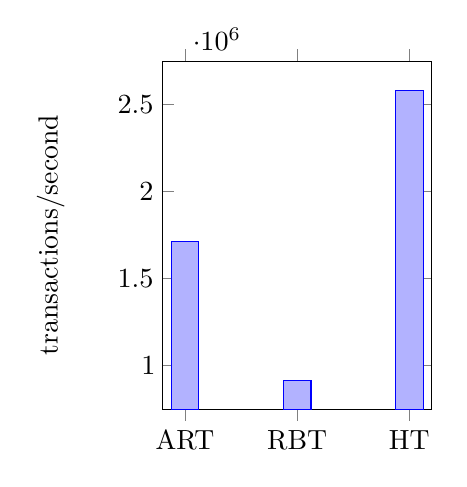
\begin{tikzpicture}
      \begin{axis}[
        ybar,
        symbolic x coords={ART,RBT,HT},
        ylabel=transactions/second,
        width=5cm,
        height=6cm,
        ]
        \addplot coordinates {(ART,1715000) (RBT,917000) (HT,2583000)};
      \end{axis}
    \end{tikzpicture}
    \caption{Lookup}
    \label{fig:lookup-microbenchmark}
  \end{subfigure}
  \begin{subfigure}[b]{0.3\textwidth}
    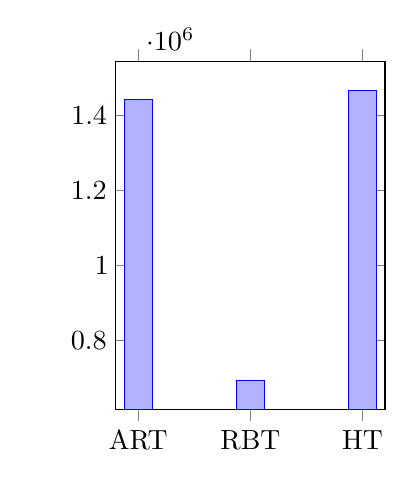
\begin{tikzpicture}
      \begin{axis}[
        ybar,
        symbolic x coords={ART,RBT,HT},
        width=5cm,
        height=6cm,
        ]
        \addplot coordinates {(ART,1441000) (RBT,695000) (HT,1467000)};
      \end{axis}
    \end{tikzpicture}
    \caption{Insertion}
    \label{fig:insertion-microbenchmark}
  \end{subfigure}
  \begin{subfigure}[b]{0.3\textwidth}
    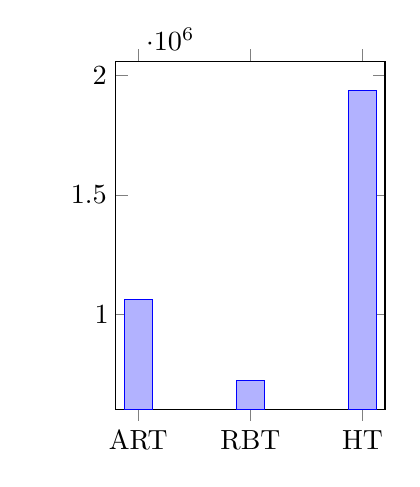
\begin{tikzpicture}
      \begin{axis}[
        ybar,
        symbolic x coords={ART,RBT,HT},
        width=5cm,
        height=6cm,
        ]
        \addplot coordinates {(ART,1064000) (RBT,725000) (HT,1939000)};
      \end{axis}
    \end{tikzpicture}
    \caption{Deletion}
    \label{fig:deletion-microbenchmark}
  \end{subfigure}
  \caption{Lookup, insertion and deletion performance of ART,
  red-black trees and hashtables.}
  \label{fig:microbenchmark}
\end{figure}

\subsection{Main Benchmark}
\label{sec:main-benchmark}

We now conduct a benchmark which assesses the transactional throughput of 
a well defined workload applied on each of the three data structures.

The more than twelve million keys used during the benchmark have structure
and do resemble paths of a hierarchy (e.g.\ ``\texttt{/a}'', ``\texttt{/a/b}'',
``\texttt{/a/c}'', etc.). The keys are ordered in reverse level order and
during each transaction we draw a key under the Zipf distribution.

We query against the randomly drawn key, and if the query returns no results,
i.e.\ the key does not exist, we insert the key, otherwise we delete it.

As \Cref{fig:main-benchmark} shows, ART performs as good as the red-black tree and the
hashtable clearly outperforms its competitors.

\begin{figure}[H]
  \centering
  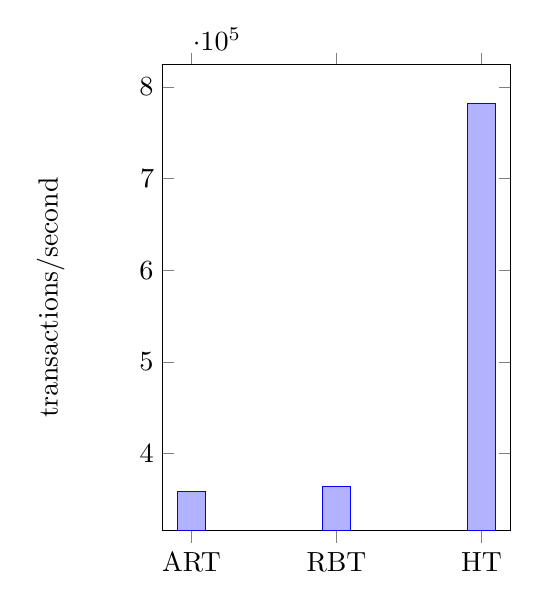
\begin{tikzpicture}
    \begin{axis}[
      ybar,
      symbolic x coords={ART,RBT,HT},
      ylabel=transactions/second,
      width=6cm,
      height=7.5cm,
      ]
      \addplot coordinates {(ART,358000) (RBT,364000) (HT,782000)};
    \end{axis}
  \end{tikzpicture}
  \caption{Transactional throughput of ART,
    red-black trees and hashtables over a skewed worload with
    mixed reads and writes.}
  \label{fig:main-benchmark}
\end{figure}

\subsection{Vertical Compression}
\label{sec:compression-benchmark}

Our last experiment measures how often vertical compression is applied.
As mentioned in \Cref{sec:vertical-compression} when deleting a node with
a single sibling, the sibling is compressed, i.e.\ merged with its parent.

If each transaction only deletes one existing key, the number of compressions
cannot exceed the number of transactions. The number of compressions
depends on span $s$. If $s=1$, every node must have exactly one sibling,
and therefore $\text{\#compressions}=\text{\#transactions}-1$. Deleting the
root node during the last step requires no compression. ART has a span of $s=8$
and we therefore do not expect a compression for every deletion.

Results should also vary depending if keys are sparse or dense. Dense keys
likely share common substrings and as a result tries require less nodes to 
store the keys. Less nodes imply a smaller number compressions. In our 
benchmark, we use sparse keys and therefore do not expect less compressions.

Figure X depicts number of compressions over number of transactions.

\section{Future Work}
\label{sec:future-work}

In this project we achieved correctness but left potential for improvements.

Our implementation uses C++ dynamic arrays, i.e. \texttt{std::vector} in order
to store compressed paths, which requires $24 + n$ bytes, where $n$ is the
number of compressed nodes. Using C-style arrays, nodes require only $16 + n$
bytes to support vertical compression.

We also plan to optimize commonly used procedures, e.g.\ prefix checking
against a search key or child node lookup/modification by leveraging the vastly
faster C++ standard library array comparison and modification methods
(e.g.\ \texttt{memcmp}, \texttt{memset}) and try avoiding loops.

Leis et al.\ use \textit{hybrid} vertical compression, i.e.\ only store the
8 first bytes of the compressed path in a static array and the number of
compressed nodes. We use pessimistic vertical compression, which stores
the entire compressed path.
Their approach leverages on-CPU caches since it decreases memory fragmentation
but keys must be stored at the leaves and one additional comparison is
required at the leaf node. We want to know how strong we benefit from hybrid 
vertical compression and how much it impacts memory consumption.

Finally, our implementation dictates single threaded usage, but we intend to
incorporate concurrency control in order to further increase the transactional
throughput of ART when multiple cores are present.

\newpage

\bibliographystyle{abbrv}
\bibliography{art}

\end{document}
